% !TEX root = Konzept.tex
\chapter{Game Design}
Um unsere Gedanken zur Spielidee niederzuschreiben, erstellten wir ein digitales Whiteboard bei Miro, um über einen einfachen und direkten Weg Ideen zu teilen und festzuhalten. Um hierbei die Wahl der Konzepte nicht bereits im Vorhinein zu stark einzuschränken, wurde eine sehr offene und erweiterbare Spielform in Form eines \textit{Escape Rooms} als Grundlage gewählt. Diese Idee wurde im Laufe der Entwicklung spezifiziert und stetig verändert, jedoch blieb erhalten, dass ein Spieler Puzzle und Aufgaben verschiedener Arten lösen muss, um aus dem Ort im dem der Spieler gefangen ist zu entkommen und somit das Ende des Spiels zu erreichen. Dies bot die Freiheit, mit vielen verschiedenen Ideen zu arbeiten, welche verschiedene Grundkonzepte der Interaktion ansprachen. Das finale Konzept der Spielidee wird im Folgenden beschrieben.

\section{Spielidee}
Der Spieler findet sich in einem magischen Turm wieder, in welchem alle Farben verschwunden sind. Ohne Farben existiert kein Leben in diesem Turm, weshalb alles starr und unbenutzbar ist. Jedoch sind in diesem Turm Farbkristalle verteilt, mit welchen man die Farbe wieder in die Welt freilassen kann. Das Ziel ist es, diese farblose Welt im Verlaufe des Spiels Rätsel-für-Rätsel einzufärben und die Farben zu nutzen um den Turm zu erklimmen und ihm letztendlich zu entkommen.

\section{Setting, Look \& Feel}
Der Look des Spiels orientiert sich, wie die Spielidee bereits vermuten lässt, optisch an einer magischen, rätselhaften Welt. Da die Farbkristalle im gesamten Turm verteilt sind, existieren neben der Farbe Weiß nur noch die primären Farben des subtraktiven Farbschemas (CMYK) Cyan, Magenta, Gelb und Schwarz (Key). Entlang dieser Farben, ist das Innere des Turms in separierte Räume unterteilt, in welchen je ein Stein zu finden ist. Diese Räume haben die Farbe des Steines angenommen, welcher in ihnen liegt. Damit fällt die Orientierung im Turm dem Spieler leicht, da er immer ein klares Ziel vor Augen hat. Jedem dieser Bereiche wurden eigene Themen zugewiesen, welches die Farbe des Raumes präsentiert und eine Vielzahl an Rätseln beherbergt. Im Folgenden werden die Räume kurz erklärt.
\newpage
\noindent
\subsection{Lobby}
Die Lobby symbolisiert den Bereich des Spiels, zu welchem der Spieler einige Male zurückkehren wird. Da dieser Raum an alle weiteren Farbräume grenzt, sollte er das Setting des Spiels als Ganzes aufgreifen. Somit ist die Lobby ein Raum, der mit magischen oder zur Herstellung magischer Objekte wie Pflanzen und Erzen, dekoriert ist. Zusätzlich zu diesem allgemeinen Magie-Thema behandelt der Raum das Thema Alchemie, mit welchem ein Spieler über das Rätsel des Raums in Kontakt tritt. Bei diesem muss ein Spieler Tränke in der richtigen Farbe brauen, damit die gebraute Farbe wieder in die Welt freigelassen werden kann. Um zu den Farbräumen zu kommen, hat die Lobby eine Vielzahl von Treppen, welche in die richtige Position gebracht werden müssen um den Weg zu den jeweiligen Räumen zu eröffnen.

\subsection{Cyan-Raum}
Der Cyan-Raum verkörpert als erster Farbraum des Spiels das Thema \dq Werkstatt\dq. In diesem Raum befinden sich neben üblichen Handwerksmaterialien, Konstrukte wie eine Uhr und Zahnräder. Dies bietet das Gefühl eines Uhrwerks. Hinzu kommt das Rätsel des Raums, bei welchem man Röhren an einer Wand befestigen muss. Hierbei soll dem Spieler erneut das Gefühl gegeben werden, dass dieser Raum zum Schaffen und Werkeln gedacht ist. Abgerundet wird der Raum durch eine dekorierte Golfbahn, um sich etwas von der Arbeit zu erholen.

\subsection{Magenta-Raum}
Im Magenta-Raum befinden sich Bücher, Leitern und große Tische. Diese Kombination von Objekten soll das Thema \dq Bibliothek\dq betonen. Der Raum bietet zwei Minispiele: im ersten Minispiel fordert es Geschick und Können, da der Spieler hier eine Murmel in einer Box durch Neigung in ein Loch navigieren muss. Im zweiten Minispiel wird ein Rätseltisch thematisiert, dessen Tricks ein  Spieler verstehen muss um den Farbkristall zu erhalten.

\subsection{Gelb-Raum}
Der letzte Raum des Spiels ist der Gelb-Raum. Um in diesem Raum für Abwechslung zu sorgen, fehlt hier die Beleuchtung fast vollständig. Der Raum befasst sich mit Astronomie, Astrologie und arkanen Künsten. Mithilfe von Leuchtstäben muss ein Spieler hier selbst für Licht sorgen, um die Geheimnisse des Raums zu lüften und damit das Rätsel zu lösen.

\newpage
\noindent
\section{Spielbeginn}
\begin{wrapfigure}{r}{6cm}
	\vspace*{-0.5cm}
	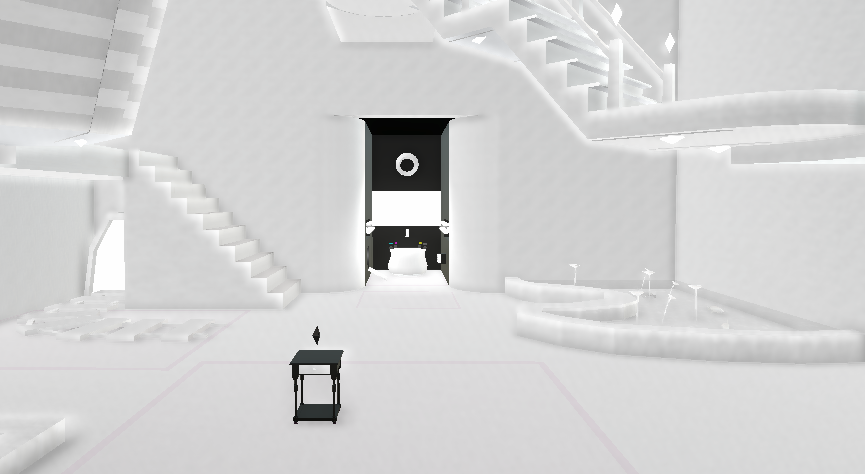
\includegraphics[width=5.9cm]{Pictures/Lobby_Start}
	\caption{Spielwelt zu Beginn}
	\vspace*{-0.5cm}
	\label{fig:spielwelt-beginn}
\end{wrapfigure}

Zum Spielbeginn befindet sich der Spieler in der Lobby, welche den Hauptbereich des Spiels darstellt. Hier wird dem Spieler aufgrund fehlender Farbe ein erster Eindruck vom erdrückenden Weiß, sowie der Größe des Turms gegeben. Der Raum enthält außerdem direkt den ersten schwarzen Farbkristall, welcher als eine Einführung in die Mechaniken des Spiels dient. Dieser kann also direkt im Alchemie-Rätsel benutzt werden. Dazu aber in einem späteren Kapitel mehr.\\

\section{Spielfortschritt}
Um im Spiel Fortschritt zu erzielen, muss ein Spieler die Rätsel der einzelnen Farbräume lösen und die daraus gewonnenen Farbkristalle im oben erwähnten Alchemie-Rätsel in der Lobby in Farbe konvertieren, um so die verschiedenen Farben in die Spielwelt zurückzubringen.
Aufgrund des Aufbaus des Treppenrätsels müssen die Räume in einer festgesetzten Reihenfolge durchgespielt werden. Die Treppen sind durch Farben markiert, welche freigesetzt werden müssen, bevor eine jeweilige Treppe bewegt werden kann.

\section{Spielende}
Sobald alle Farben in die Welt freigelassen wurden, ist die Lobby vollends eingefärbt. Damit können auch alle Treppen bewegt werden, welche in einem letzten Rätsel in einer speziellen Reihenfolge angeordnet werden können, um es dem Spieler zu ermöglichen höher zu klettern als er je zuvor konnte. Sobald der Spieler oben angekommen ist und eine letzte Leiter erklommen hat, kann er einen Schlüssel greifen und mit diesem die Eingangstür des Turms öffnen. In diesem Zuge entkommt der Spieler aus dem Turm und hat das Spiel vollendet.


\chapter{Umsetzung}
Doch was genau wurde letztendlich umgesetzt? Dies soll im folgenden Kapitel genauer erläutert werden.

\section{Bewegung im Spiel}
\begin{wrapfigure}{r}{6cm}
	\vspace*{-0.5cm}
	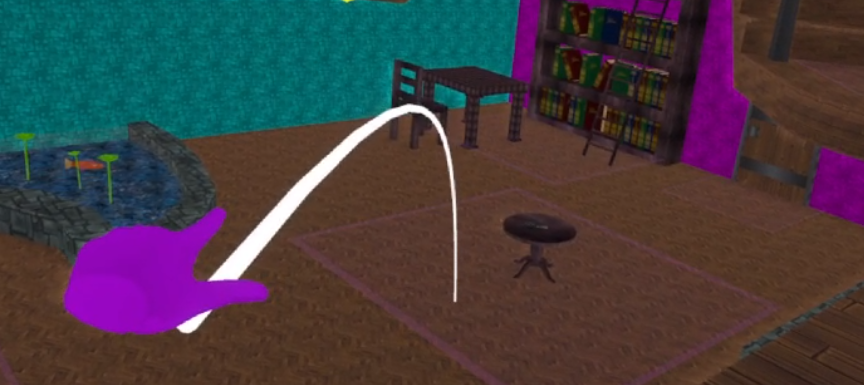
\includegraphics[width=5.9cm]{Pictures/Bewegung}
	\caption{Bewegung}
	\vspace*{0cm}
	\label{fig:bewegung}
\end{wrapfigure}

Da dieses Projekt keinen Wert auf schnelle Bewegungen, sondern viel eher auf gute Spielerfahrungen und das Lösen von Rätseln ohne Zeitdruck legt, wurde sich für die Teleport-Fortbewegung und Raster-Drehung entschieden. Diese Entscheidung hat das Ziel, Motion Sickness erheblich vorzubeugen. Zusätzlich wurden festgesetzte Teleportationsbereiche definiert, um die Bewegung des Spielers durch die jeweiligen Räume zu kontrollieren und somit sicherzustellen, dass ein Spieler die relevanten Bereiche eines Raumes erkennt und nicht allzu sehr von der Umgebung abgelenkt oder verwirrt wird. Ein Spieler hat somit die Möglichkeit, mit dem Joystick der VR-Controller einen Laser zu erzeugen, welcher zunächst rot hervorgehoben wird. Sollte ein Laser das erste Mal in einen Teleportationsbereich hineingehalten werden, färbt sich dieser weiß. Das Loslassen des Triggers führt anschließend dazu, dass sich die Position des Spielers auf den Schnittpunkt zwischen Laser und Teleportationsbereich setzt. Die einzige Ausnahme bilden hierbei die Teleportationsbereiche der Treppen. Sollte sich ein Spieler auf Treppenstufen teleportieren wollen, so ändert sich die Position abhängig vom Laser auf den nächstgelegenen geebneten Bereich der Treppe anstatt auf der Schräge der Treppen zu stehen.\\
Da die Erreichbarkeit von Treppen im Treppenrätsel von der Position der Treppe abhängt, dürfen die Teleportationsbereiche es einem Spieler nicht ermöglichen über Abgründe zu teleportieren. Um dies zu vermeiden, werden ausschließlich Teleportationsbereiche, die relativ zu der Position des Spielers valide sind, aktiviert. 


\section{Treppen}
\begin{wrapfigure}{r}{6cm}
	\vspace*{-0.5cm}
	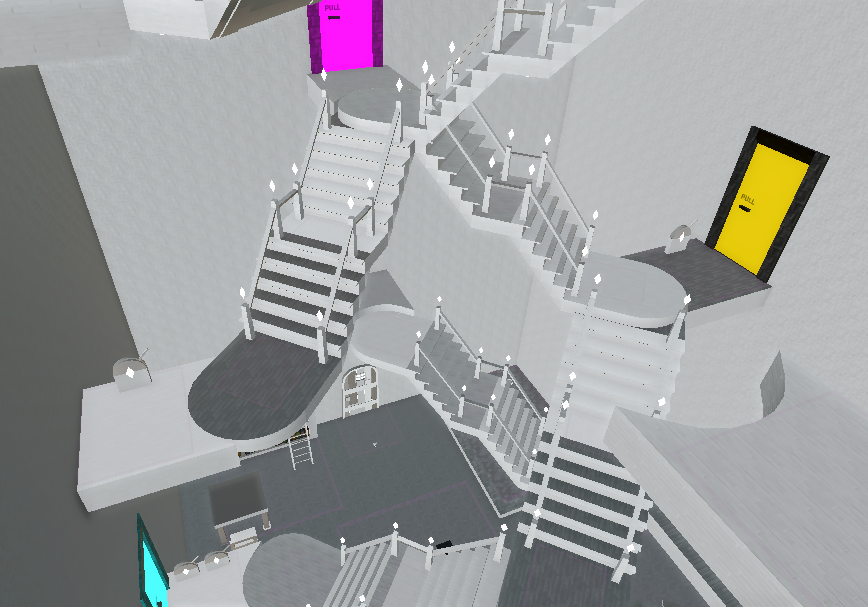
\includegraphics[width=5.9cm]{Pictures/Treppenhaus}
	\caption{Treppenhaus}
	\vspace*{-1cm}
	\label{fig:treppenhaus}
\end{wrapfigure}
\subsubsection{Erläuterung}
Die Treppen der Lobby sind durch bis zu zwei verschiedene Farben in Form von Farbkristallen markiert. Des Weiteren sind in diesem Treppenhaus Hebel verteilt, welche ebenfalls die Farbe eines Farbkristalls auf sich markiert haben. Sobald die Farbe eines Kristalls in die Welt zurückgebracht wurde, werden die Markierungen eingefärbt und die Funktionalität der Hebel und Treppen wird aktiviert. Wenn ein Hebel benutzt wird, werden alle Treppen, welche die Farbe dieses Hebels tragen von ihrer aktiven Position in die anliegende Position bewegt. Jede Treppe hat dabei eine linke und eine rechte Position. Die Ziele, welche über die Veränderungen von Treppen erreicht werden sollen, sind die farbigen Türen. Aufgrund der Positionierung und Farbgebungen der Treppen, gibt es nur einen möglichen Ablauf durch das Treppenhaus. Erst muss die Farbe Schwarz in die Welt gelassen werden, um daraufhin den Cyan-Raum zu erreichen. Mit der Cyan-Farbe kann der Magenta-Raum erreicht werden und daraufhin mit der Magenta-Farbe der Gelb-Raum. Mit allen Farben kann letztendlich der Schlüssel erreicht werden, mit welchem das Spiel beendet werden kann.


\subsubsection{Interaktion}
\noindent Die Aktion des Ziehens eines farbigen Hebels führt direkt zu der Reaktion einer Auswahl gleichfarbiger Treppen, welche im Treppenhaus zu neuen Positionen rotieren. Hier zeigt sich die Stärke des Interaktion mit einer VR-Umgebung besonders, da ein Spieler nach dem Benutzen eines Hebels direkt um ihn herum die Auswirkungen dieser Aktion spürt. Verstärkt durch das Gefühl der Höhe, welche sich zuspitzt je höher das Treppenhaus erklungen wird, ist es ein sehr imposantes und emotional ergreifendes Minispiel.

\newpage

\section{Alchemie-Puzzle}
\subsubsection{Erläuterung}
\begin{wrapfigure}{r}{6cm}
	\vspace*{-0.5cm}
	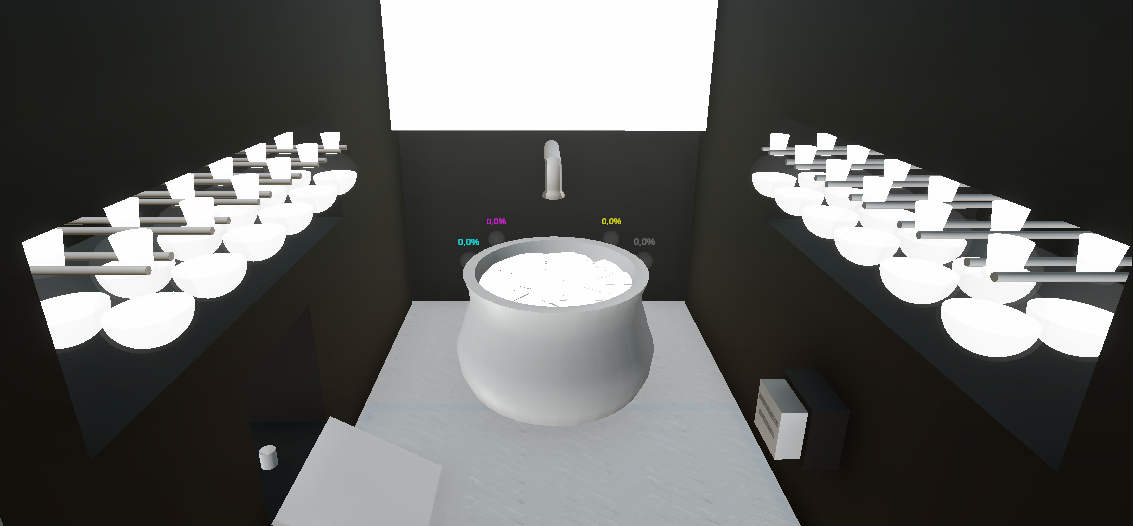
\includegraphics[width=5.9cm]{Pictures/Alchemie}
	\caption{Alchemie-Puzzle zu Beginn}
	\vspace*{-0.5cm}
	\label{fig:alchemie_start}
\end{wrapfigure}
Wie bereits in einem oberen Kapitel erwähnt, beschäftigt sich die Lobby mit dem Alchemie-Thema und bringt dabei ein Rätsel mit sich, welches der Spieler immer dann spielen wird, wenn er einen Kristall in die installierte Maschine platziert. Sobald das Spiel beginnt, wird der Kessel vor dem Spieler mit der Farbe des jeweiligen Farbkristalls gefüllt. Rechts und links vom Spieler sind Tränke in greifbarer Nähe. Insgesamt gibt es zwölf Tränke welche im Verlauf des Spiels verschiedene Farben annehmen werden. Im ersten Spieldurchlauf mit dem schwarzen Farbkristall, sind ausschließlich weiße und ein schwarzer Trank vorhanden. Sobald ein Trank in den Kessel geworfen wird, färbt sich die Farbe innerhalb des Kessels zu einer Mischfarbe zwischen der vorherigen Kesselfarbe und der Trankfarbe. Die CMYK-Werte dieser Mixtur werden in der Nähe des Kessels in Form von prozentualen Werten dargestellt.\\
Das Ziel des Spiels ist es, die Tränke zu nutzen um eine Kesselfarbe zu mischen, die mit einer im Blickfeld des Spielers dargestellten Farbe übereinstimmt. Es müssen insgesamt pro Farbkristall drei Farben gemischt werden. Sobald dies geschafft ist, entleert der Kessel sich und die Farbe des Farbkristalls wird mit einer großen farbigen Rauchwolke in die Welt geschossen. Diese Rauchwolke färbt nicht nur die umliegende Lobby und die Elemente des Treppenrätsels ein, sondern auch drei der vorerst weißen Tränke. Die Farbe jedes Farbkristalls hat drei Tränke: die Originalfarbe, eine hellere Farbe, und eine dunklere Farbe, welche in späteren Iterationen des Alchemie-Rätsels genutzt werden müssen um komplexere Farbkombinationen zu mischen.
\subsubsection{Interaktion}
\begin{wrapfigure}{r}{6cm}
	\vspace*{-0.5cm}
	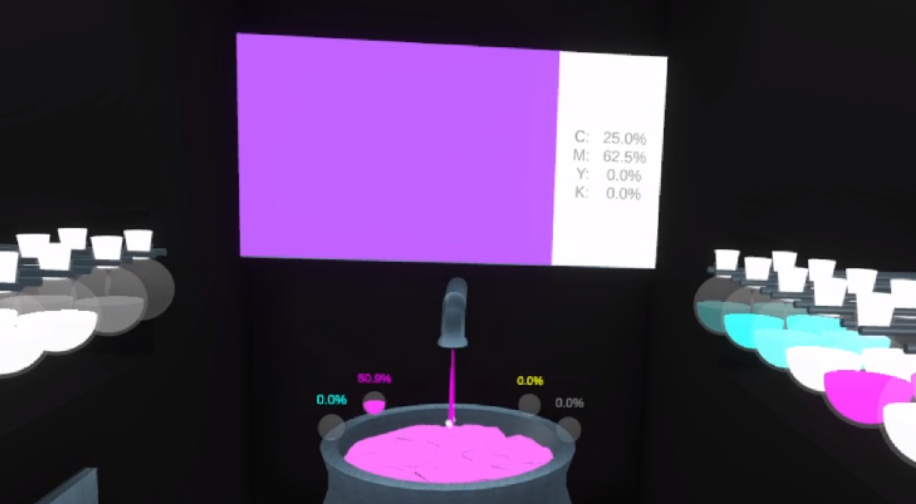
\includegraphics[width=5.9cm]{Pictures/Alchemie_Magenta}
	\caption{Alchemie-Puzzle in Magenta Iteration}
	\vspace*{-0.5cm}
	\label{fig:alchemie_magenta}
\end{wrapfigure}
In diesem Rätsel werden alle drei bereits erläuterten Formen der Interaktion verwendet um ein ansprechendes Rätsel zu erschaffen.\\
Die visuelle Interaktion zeigt sich in den Farben der Kesselflüssigkeit, des Displays und der Tränke. Ein Spieler muss die Trankfarben nutzen um die Farbe der Kesselflüssigkeit auf die Farbe des Displays anzugleichen.\\
Sobald ein Trank in den Kessel geworfen wird, werden die Farben von Trank und Kesselinhalt vermischt. Sollte die Farbe korrekt, oder der \dq Reset\dq-Button gedrückt worden sein, aktiviert die Maschine sich automatisch und setzt die Kesselfarbe zurück. Diese Form der Interaktion wird abgerundet, sobald eine Iteration des Rätsels gelöst wurde und die Farbe in die Welt zurück kommt. Erst wird der Spieler von einem Farbrauch umgeben, der ihn komplett umhüllt und sobald der Rauch schwindet wird der Spieler herausfinden, dass die Umgebung sich entsprechend neu eingefärbt hat. Das Rätsel zu lösen hat somit direkten greifbaren Einfluss auf die Umgebung des Spielers.\\ \newpage
\noindent Die haptische Interaktion wird durch das greifen und werfen der Tränke dargestellt. Anstatt Farben auszuwählen und beispielsweise durch einen einfachen Knopfdruck hinzuzufügen, wird hierbei Wert darauf gelegt, dass ein Spieler das Gefühl bekommt selbst die Tränke zu werfen und zu mixen. Dies bietet eine weitaus stärkere Integration des Spielers in die Mechaniken des Rätsels.\\
Sollte ein Spieler das Gefühl haben, einen falschen Trank benutzt zu haben, so hat er die Möglichkeit, das aktuelle Gemisch über einen Reset-Button auf der rechten Seite zurückzusetzen.\\
Da man im Spiel vier Kristalle findet, kann man dieses Minispiel bis zu vier Mal spielen, bis man die gesamte Umgebung vollständig eingefärbt hat und das Endziel erreichen kann.

\begin{figure}[h]
	\centering
	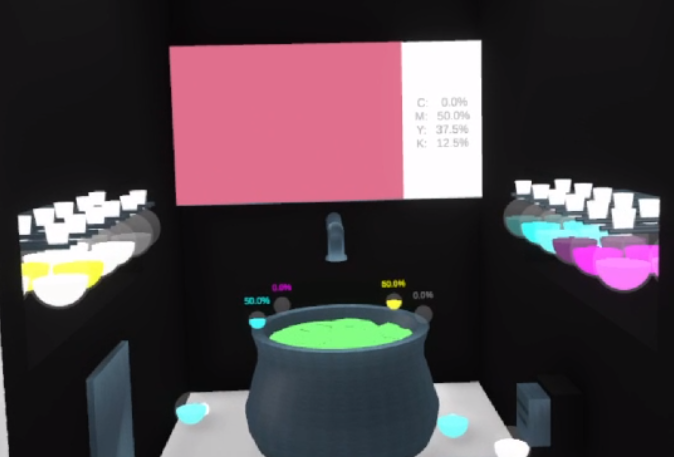
\includegraphics[width=\textwidth/2]{Pictures/Alchemie_Final}
	\caption{Alchemie-Puzzle in gelber Iteration}
	\label{fig:alchemie_final}
\end{figure}\newpage \noindent

\section{Röhren-Puzzle}
\subsubsection{Erläuterung}
Nachdem ein Spieler das erste Alchemie-Rätsel absolviert hat, ist er in der Lage, den Cyan-Raum zu erreichen. In diesem befindet sich eine Vorrichtung aus ein paar wenigen Röhren. Durch eine leichte transparente Gitter-Struktur in der Wand soll dem Spieler vermittelt werden, dass herumliegende Röhren in dieser zu platzieren sind. Die Objekte befinden sich beim ersten Berührungspunkt mit dem Spieler in einer Kiste, aus welcher sie dann aufgehoben werden können. Da Anfang und Ende des Puzzles bereits fest installiert sind, sollte der Spieler eine Auffangschale rechts neben dem Start bemerken. In der Nähe dieser wird über einen Hinweis bereits angedeutet, dass hier ein Gegenstand empfangen werden kann. Beim genaueren Verfolgen der Röhren sollte man schlussfolgern, dass sich der blaue Kristall in den waagerechten Röhren oberhalb des Spielers befindet. Um ihn zu erreichen, muss man also einen Durchfluss ermöglichen. Dazu hat man jedoch nur begrenzt viele Rohre. Diese lassen sich dabei in zwei Kategorien mit je zwei Variationen unterscheiden. In der Vorrichtung befinden sich nämlich gewinkelte sowie gerade Röhren, welche frei bewegt und platziert werden können. Hinzu kommen bereits fest installierte, welche lediglich hinsichtlich ihrer Rotation angepasst werden können. Dies wird dem Spieler über Rotationspfeile auf den Gegenständen präsentiert. Nach jeder Platzierung prüft der Manager des Rätsels, ob das Ende der Röhren vom Start ausgegangen ohne Lücken erreicht werden kann. Technisch betrachtet lässt sich sagen, dass ein Rohr in diesem Spiel bis zu zwei Nachbarn haben kann, welche über Collider gesetzt werden können. Somit lässt sich die Iteration über platzierte Röhren als verkettete Liste betrachten, da ein Rohr seine Nachbarn kennt.\\
\begin{wrapfigure}{r}{6cm}
	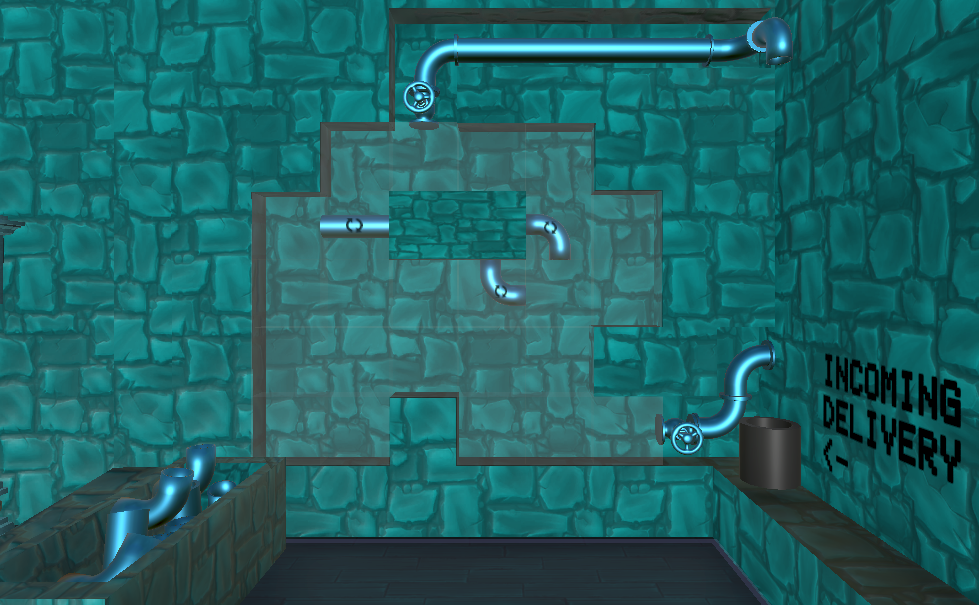
\includegraphics[width=5.9cm]{Pictures/Roehren}
	\caption{Murmelbox}
	\vspace*{-1cm}
	\label{fig:cyan}
\end{wrapfigure}
\subsubsection{Interaktion}
Wenn eine Röhre in die Gitterstruktur gehalten wird, erscheint dem Spieler eine transparente und korrekt positionierte Preview der Röhre, an welcher sie platziert werden würde, sollte man sie loslassen. Die Preview hat dabei eine von vier möglichen Rotationen, welche anhand der Rotation des Rohrs ermittelt wird. Diese Reaktion der Umgebung vermittelt dem Spieler direkt, dass Röhren exakt hier platziert werden können. Analog dazu nimmt eine Röhre die Position und Rotation der zuvor sichtbaren Preview ein, sobald sie platziert wurde. Außerdem schaltet sich bei allen Röhren, welche den weiteren Durchfluss gewährleisten, ein Licht an, um dem Spieler Feedback darüber zu geben, ob er die Verbindung richtig gesetzt hat. 
\\ \noindent Der Trick an diesem Rätsel ist die Begrenzung der Möglichkeiten durch die feste Anzahl an zu platzierenden Röhren und der Variation aller zuvor platzierten Rohre, welche lediglich rotiert werden können. Dadurch ergibt sich nach genaueren Überlegungen anhand gegebener Mittel eine einzige Lösung, zu welcher man nur durch Überlegen und Ausprobieren kommt. Dieses Konzept beschreibt eine weitere visuelle Interaktion, da man nur durch Betrachten seiner Mittel und der Gitter-Struktur auf eine Lösung kommen kann. Umgebungsinteraktion erfährt der Spieler außerdem dadurch, dass sich beim Abschluss des Rätsels, wenn der Durchfluss vollständig ist, die Farbe im Rohr\-system aktiviert, wodurch die Farbe den Kristall herausströmt.
\newpage

\section{Murmelbox}
\subsubsection{Erläuterung}
\begin{wrapfigure}{r}{6cm}
	\vspace*{-0.5cm}
	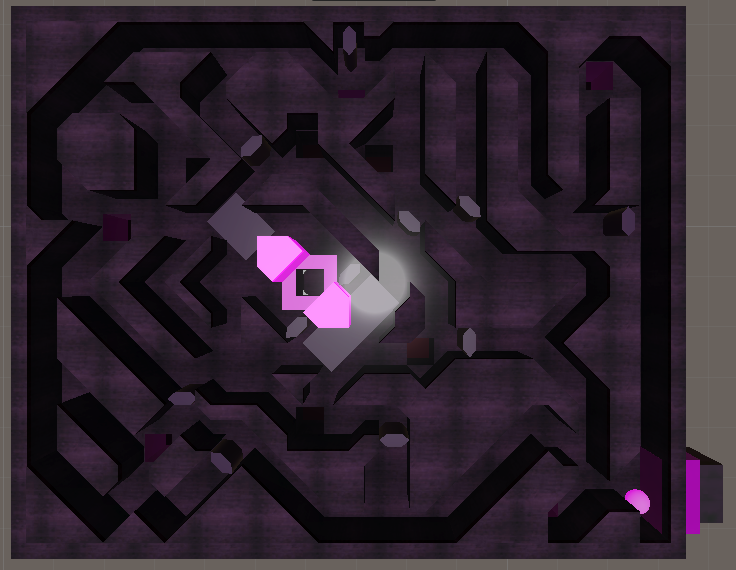
\includegraphics[width=5.9cm]{Pictures/Murmelbox}
	\caption{Murmelbox}
	\vspace*{-0.5cm}
	\label{fig:murmelbox}
\end{wrapfigure}
Im Murmelbox-Rätsel des Magenta Raums, geht es um das Feingefühl des Spielers. Wie der Name bereits aussagt, handelt es sich hier um eine Box, in der eine Murmel enthalten ist. Der Spieler kann von oben aus in diese Box hinein schauen und mithilfe zweier Hebel die Neigung der Box nach rechts, links, hinten und vorne ändern. Das Ziel des Spiels ist es durch das Kippen und Neigen der Box die Murmel in ein markiertes Loch in der Mitte zu befördern. Dies wird jedoch durch einen labyrinthartigen Parkour mit anderen \dq falschen\dq Löchern erschwert. Genannte Löcher setzen die Murmel auf eine feste Startposition zurück, sorgen jedoch auch genau die vorhandene Druckplatten dafür, dass damit bestimmte Wände entfernt bzw. hinzugefügt werden, wodurch die Spielfläche vereinfacht wird und mehr Möglichkeiten bietet um zum Ende zu kommen. Die Murmel kann außerdem über einen \dq Reset-Button\dq manuell auf die Startposition gesetzt werden, um schneller aus misslichen Lagen wieder heraus zu kommen.


\subsubsection{Interaktion}
\noindent Die Haptische Interaktion der Murmelbox war ursprünglich so geplant, dass man die Box mit der Hand greift und sie somit rotiert. Diese Form der kinematischen Bewegung war jedoch nicht mit dem derzeitigen System nicht kompatibel wodurch das haptische Feedback und die Steuerung des Spiels nun über das greifen der Hebel, zum gleichzeitigen Neigen der Box in entsprechende Richtungen, passiert. Hierbei hat der Spieler auf seine Hand- und Armbewegungen zu achten, da diese zum Neigen bzw. Kippen und dadurch zum Bewegen der Murmel essentiell sind.\\

\noindent Visuelle Interaktion erhält der Spieler durch die sich bewegende Murmel, welche sich farblich vom Boden abhebt. Dafür kann der Spieler sich einen Weg überlegen und einsehen, um diesen dann mit der Murmel zurück zu legen.

\noindent Umgebungsinteraktion bekommt der Spieler durch die sich anpassenden Wände, beim Fallen in ein falsches Loch oder beim berühren einer Druckplatte. Hier hat das Spielen und navigieren der Kugel in ein falsches Loch die Auswirkung, dass dadurch leichtere Wege zum Ziel genommen werden können wohingegen Druckplatten dafür sorgen, dass das Spiel durch geöffnete bzw. wieder geschlossene Wände erschwert wird. Weiteres Feedback erhält man durch das Abschließen des Spiels, wobei das Licht, welches den Murmelboxbereich erhält ausgeht und somit zeigt, dass das Murmelspiel beendet und damit nicht mehr relevant für den Raum ist.\\
\newpage


\section{Rätseltisch}
\subsubsection{Erläuterung}
Der Rätseltisch bildet das zweite Rätsel des Magenta Raums und lässt sich in 4 Bereiche, bestehend aus jeweils einem Rätsel, unterteilen. Der Spieler ist hier befähigt sich mit jedem Bereich zu jeder Zeit auseinander zu setzen, wobei eine Reihenfolge nur dadurch entsteht, dass mit einem finalen Bereich erst interagiert werden kann, wenn mindestens ein anderes Rätsel des Tischs abgeschlossen wurde.

\subsubsection{Erläuterung Rätsel 1}
\begin{wrapfigure}{r}{6cm}
	\vspace*{-0.5cm}
	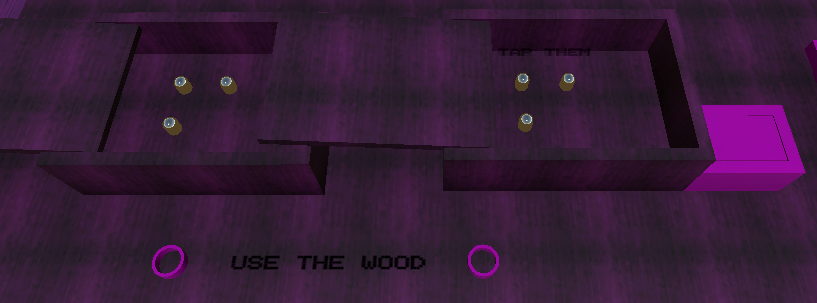
\includegraphics[width=5.9cm]{Pictures/Tisch1}
	\caption{Rätseltisch 1}
	\vspace*{-0.5cm}
	\label{fig:tisch1}
\end{wrapfigure}
Das erste Rätsel des Tischs enthält zwei nebeneinander-liegende Kisten und zwei zugehörige Fingerpodeste, die bei Interaktion den Deckel der entsprechenden Box öffnen. Sobald nicht mehr mit dem Podest interagiert wird, schließt sich die Box jedoch wieder. Jede Kiste beinhaltet jeweils drei Lichter, die vom Spieler angeschaltet werden können und beim Schließen des Deckels der zugehörigen Box wieder ausgehen. Ziel des Spiels ist alle sechs Lichter gleichzeitig zum Leuchten zu bringen, wobei der Spieler versuch muss beide Boxen gleichzeitig offen zu halten und währenddessen die Lichter anzuschalten. Um dem Spieler noch etwas an die Hand zu geben wird er hier außerdem darauf hingewiesen, etwas anderes statt nur seine Hände zu verwenden um das Rätsel zu lösen. Sobald das Spiel beendet wird öffnet sich kurz darauf die kleinere Box daneben um das Abschließen des Spiels zu signalisieren und dem Spieler ein hölzernes Plättchen mit der Aufschrift \dq P\dq zu präsentieren.\\

\subsubsection{Erläuterung Rätsel 2}
\begin{wrapfigure}{r}{6cm}
	\vspace*{-1cm}
	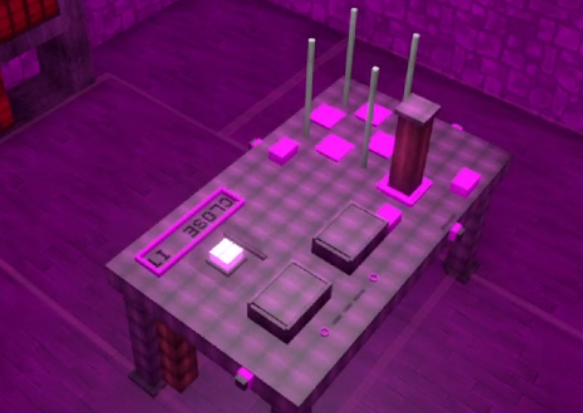
\includegraphics[width=5.9cm]{Pictures/Tisch2}
	\caption{Rätseltisch 2.1}
	\vspace*{0cm}
	\label{fig:tisch2}
\end{wrapfigure}
Das zweite Rätsel besteht aus einem Holzturm mit greifbarem Ring. Um den Tisch verteilt an jeder Tischkante sind insgesamt vier Knöpfe, die beim Drücken dafür sorgen, dass die Fortschritts anzeige, welche am Holzturm dargestellt wird, um eine Sektion nach oben fährt. Das Ziel des Spiels bildet hierbei das Drücken aller vier Knöpfe, um den Fortschritt am Holzturm bis oben hin zu füllen. Lässt man einen Knopf jedoch los fällt der Fortschritt wieder. Hierbei kann der Spieler die Fortschrittsanzeige mithilfe des Rings am Holzturm an bestimmten Punkten festsetzen, wodurch der Fortschritt nicht mehr fällt, bis man den Ring wieder vom aktuellen Fortschrittsstand weg bewegt. Nach abschließen des Spiels öffnet sich kurz darauf auch hier die nebenstehende kleine Box wodurch der Spieler das nächste hölzerne Plättchen mit der Aufschrift \dq N\dq erhält\\
\newpage

\subsubsection{Erläuterung Rätsel 3}
\begin{wrapfigure}{r}{4cm}
	\vspace*{-1.5cm}
	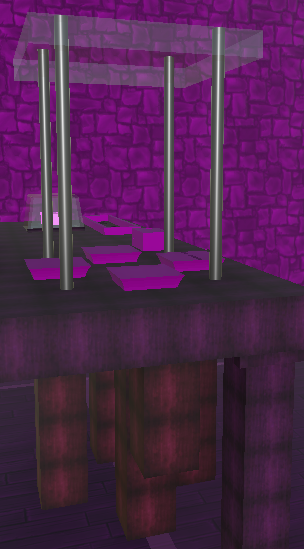
\includegraphics[width=4cm, height=6cm]{Pictures/Tisch3}
	\caption{\\ \noindent Rätseltisch 3}
	\vspace*{-1cm}
	\label{fig:tisch3}
\end{wrapfigure}
Das dritte Rätsel besteht aus 4 Holztürmen die am Spielbeginn noch an der untersten Position im Tisch stecken. Diese Türme sind vom Spieler greif- und nach oben verschiebbar. Ziel des Spiels ist es die richtige Sequenz herauszufinden auf welcher Höhe die Türme stehen müssen und diese entsprechend zu stellen. Die Platzierung der Türme nach unten hin, wird durch die vorhanden Holztürme an den jeweiligen Tischkanten dargestellt. Nachdem das Rätsel gelöst wurde und die Türme entsprechend platziert, öffnet sich hier ebenfalls die kleine Box daneben und gibt damit Zugriff das nächste hölzerne Plättchen ohne Aufschrift.\\

\subsubsection{Erläuterung Finales Rätsel}
\begin{wrapfigure}{r}{4cm}
	\vspace*{-0.7cm}
	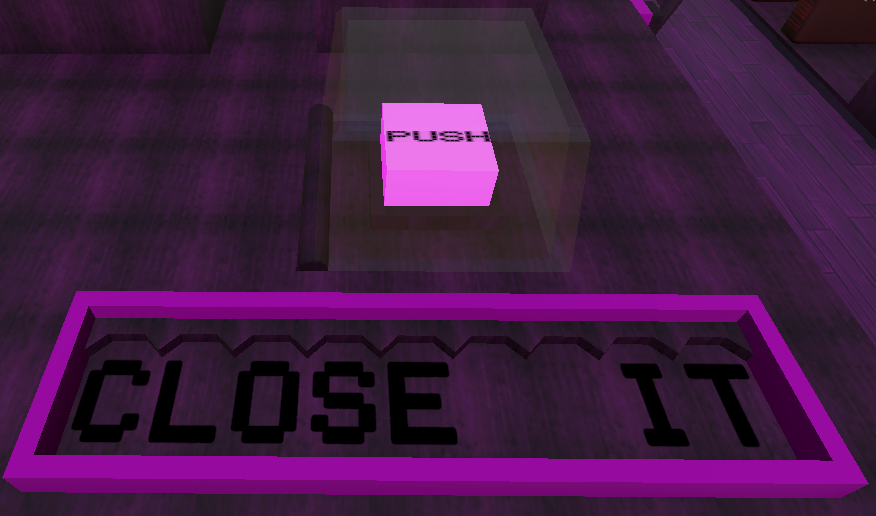
\includegraphics[width=4cm]{Pictures/Tisch4}
	\caption{\\ \noindent Rätseltisch Finale}
	\vspace*{-0.2cm}
	\label{fig:tisch4}
\end{wrapfigure}
Der letzte Bereich des Tisches besteht aus einem Kopf mit der Aufschrift \dq PUSH\dq, der von einem Glaskasten umgeben ist und einem Sequenzfeld, in dem die Aufschrift \dq CLOSE  IT\dq abgebildet wird. Alle vorangegangenen Rätsel eröffnen nach ihrem Abschluss Zugriff auf ein hölzernes Plättchen. Außerdem liegt am unteren Ende des Sequenzfeldes ein weiteres ohne Aufschrift. Diese Plättchen können in das Sequenzfeld eingelegt werden um entsprechend die Aufschrift zu verändern. Ziel des Spiels ist es, die gezeigte Wortsequenz so zu verändern, dass sich der Glaskasten öffnet und man den Button drücken kann. Durch das Drücken des Buttons wird der Abschluss des Rätseltischs markiert, wodurch das Licht über dem Tisch entsprechend ausgeht. 

\subsubsection{Interaktion}
Der Rätseltisch hat viele klare Elemente in denen haptisches Feedback vermittelt wird. Man kann und muss zur Lösung der Rätsel mehrere Dinge wie ganze Holztürme oder Plättchen greifen, man interagiert mit Lichtern, die man durch Berührung an und ausschaltet und man hat die Aufgabe Knöpfe zu drücken, wobei hier sogar Beidhändigkeit wichtig ist, da man den Knopf drücken und andere Objekte greifen kann.\\

\noindent Visuelle Interaktion hat der Rätseltisch in Form des dritten Rätsels beim verschieben der Türme. Hierbei muss sich der Aufbau des Tischs und die entsprechenden Seiten genau angeschaut werden, um auf die korrekte Höhe und Position der Türme zu kommen.\\

\noindent Die Reaktive Interaktion des Rätseltischs ist in jedem der vier Rätsel vereint. Im ersten gibt es beispielsweise Boxdeckel, die durch Spieler-Interaktionen gesteuert werden können. In Rätsel 2 sorgt die sich sofortig anpassende Spielfortschrittsleiste dafür, dass jeder neue Knopfdruck direktes Feedback gibt und etwas verändert. Außerdem öffnet sich beim Abschließen jedes vorigen Rätsels eine kleine Box, wodurch man erst dann Zugriff auf essentielle Gegenstände bekommt sowie beim Abschließen des finalen Rätsels die Glasbox, womit man das Rätsel abschließen kann und damit ebenfalls das Licht des Rätseltischs ausgeschaltet wird.
\newpage
\noindent
\section{Gelb-Raum}
\begin{wrapfigure}{r}{6cm}
	\vspace*{-1cm}
	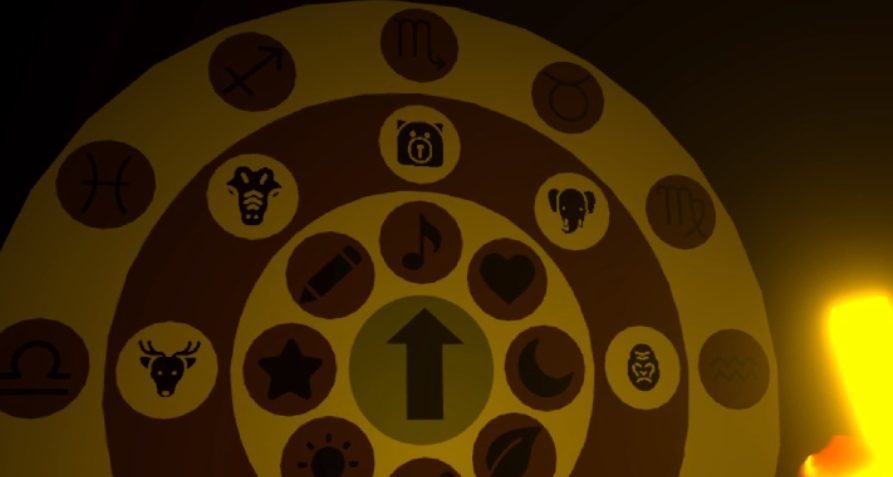
\includegraphics[width=5.9cm]{Pictures/Gelb-Raum}
	\caption{Gelb-Raum}
	\vspace*{-1cm}
	\label{fig:Gelb-Raum}
\end{wrapfigure}
\subsubsection{Erläuterung}
Im letzten Farbraum des Spiels, dem Gelb-Raum, wird dem Spieler die Fähigkeit normal zu sehen, entzogen. Mithilfe eines leuchtenden Spenders, den ein Spieler im Raum durch das starke Leuchten finden wird, kann man den Raum durch greifbare Leuchtstäbe punktuell erhellen und erforschen. Das wird auch für die Lösung des Raums benötigt. Wie bereits in einem vorherigen Kapitel erwähnt, sind die Themen des Raums Astronomie, Astrologie, Mystik und Kunst. Diese Themen tragen zusammen zur Lösung eines verstellbaren Rads bei, welches in drei Sektionen unterteilt ist. Der äußere Ring zeigt hierbei die Symbole der zwölf Sternzeichen. Abgesehen von dem Spender und seinen Leuchtstäben leuchtet lediglich ein Sternbild an der Decke, welches eins dieser zwölf Sternzeichen darstellt. Um dem Sternbild ein Zeichen zuordnen zu können, muss man im Raum eine Legende finden, die diese Beziehung aufweist. Das mittlere Segment des Rads umfasst acht Tiere, u. a. Hirsch, Tiger, Nilpferd und Bär. Alle diese vier Tiere befinden sich in Form eines Kopfes als Trophäe im Raum wieder. Um die richtige Lösung zu finden, muss man die Tierköpfe mit den Leuchtstäben gründlich erforschen, da auf der Rückseite eines Kopfes das richtige Symbol versteckt ist. Dies mag zu Beginn etwas unscheinbar sein, jedoch handelt es sich bei diesem Spiel um ein Rätsel-Spiel und die Tierköpfe sind allesamt erreichbar und auf dem Rad zu finden. Daher sollte es naheliegend sein, zu versuchen, mit ihnen zu interagieren. Das letzte Segment des Rads umfasst acht verschiedene Symbole, die teilweise Anlehnungen an Namen von Tarotkarten sind. Sollte sich der Spieler im Raum gründlich genug umschauen, so findet er ein Schränkchen mit einer Schublade, in welcher sich zuzüglich zu einem Buch eine Tarotkarte befindet. Dessen Name lässt auf das korrekte Symbol auf dem Rad schließen.
\begin{wrapfigure}{r}{6cm}
	\vspace*{-1cm}
	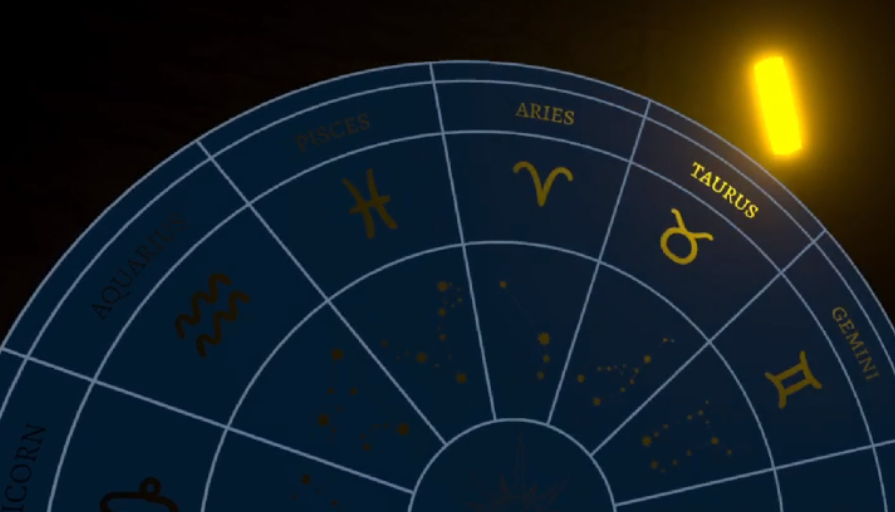
\includegraphics[width=5.9cm, height=3cm]{Pictures/Gelb-Raum_Sternenkarte}
	\caption{Sternenkarte}
	\vspace*{-1cm}
	\label{fig:Gelb-Raum_sternenkarte}
\end{wrapfigure}
\subsubsection{Interaktion}
Wie zuvor erwähnt, ist die Einschränkung der Sicht auch ein gutes Mittel, um besondere Erfahrungen mit visuellen Interaktionen zu sammeln, da der Raum die Verantwortung der Sicht auf den Spieler legt. Im Gelb-Raum muss er Lichtquellen in den Raum werfen, um die allumfassende Dunkelheit des Raumes punktuell zu durchbrechen. So etwas Fundamentales wie die Lichtverhältnisse eines Raumes in die Hand der Spieler zu legen, führt zu einer deutlichen Erhöhung der Konzentration und Immersion. Dabei fiel uns auf, dass Spieler, die damit beschäftigt waren ihren Sichtsinn aufrechtzuerhalten, intensiver in das Spiel vertieft waren.
Umgebungsinteraktionen zeigen sich, wie auch schon im Treppenhaus bei den Hebeln des Gelb-Raums wieder. Durch das Betätigen der Hebel, verstellt sich das entsprechende Segment des Rings. Weiterhin leuchtet der Pfeil des Rads hell auf und eine versteckte Wand öffnet sich, sodass der darin liegende Kristall aufgesammelt werden kann, sobald alle Segmente korrekt ausgerichtet wurden.

\newpage \noindent

\section{Spielabschluss}
\begin{wrapfigure}{r}{6cm}
	\vspace*{-0.5cm}
	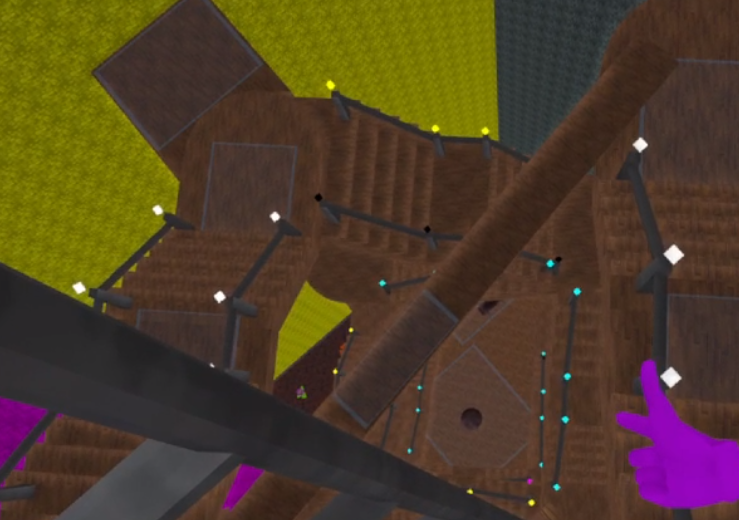
\includegraphics[width=5.9cm]{Pictures/Ausblick_Leiter}
	\caption{Ausblick Leiter}
	\vspace*{-0.5cm}
	\label{fig:leiter}
\end{wrapfigure}
Um das Spiel abzuschließen, muss der Spieler zuvor alle der vier Farbkristalle gefunden und mithilfe des Alchemie-Puzzles aktiviert haben. Damit ist er in der Lage alle Hebel des Treppenhauses zu nutzen, sodass die oberste Etage des Turms erreicht werden kann. Hier, beim höchsten Punkt des Turms, wird der Spieler vor eine weitere interessante visuelle Interaktion gestellt. Er muss auf eine dünne Planke steigen, wobei man ein freies Sichtfeld auf die Tiefe unter sich hat. Die Reaktion auf diese Höhe kann sehr individuell sein, jedoch erzeugt sie starke Emotionen.\\
Anschließend muss der Spieler eine lange Leiter hochzuklettern, um den silbernen Schlüssel zu erlangen. Nachdem er diesen aufgesammelt hat, kann er in die Lobby des Turms zurückkehren und den gefundenen Schlüssel in die Eingangstür zu stecken. An dieser Stelle erscheint ein Endbildschirm, welcher das Spiel beendet.
\begin{figure}[h]
	\centering
	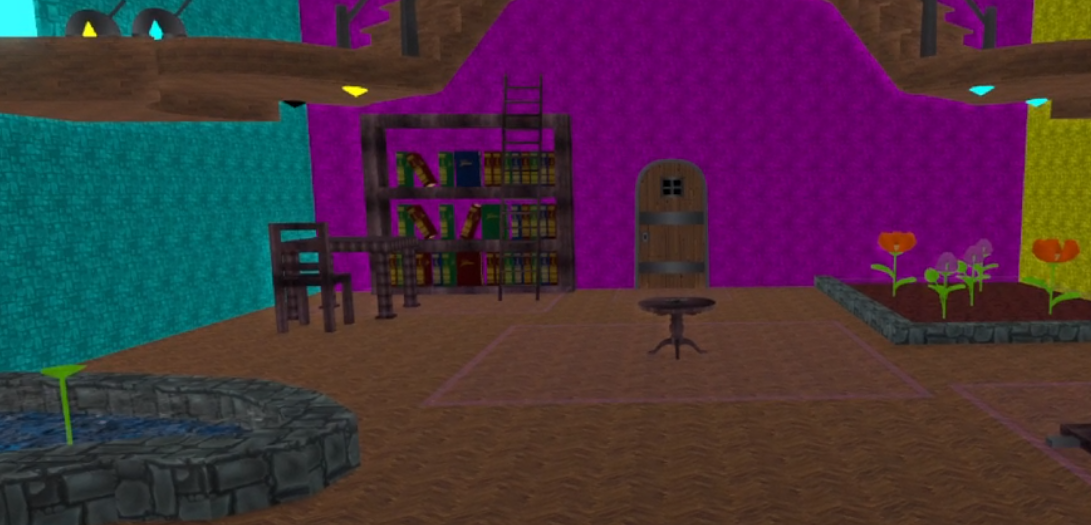
\includegraphics[width=\textwidth/2]{Pictures/Lobby_Final}
	\caption{Lobby Spielende}
	\label{fig:lobby_final}
\end{figure}
\newpage

\section{Interaktion mit Haptic Gloves}
In den vorherigen Abschnitten wurde nicht im Besonderen auf die Haptic Gloves eingegangen. Aufgrund technischer Probleme in der Anbindung der Haptic Gloves an die bereits bestehenden Funktionalitäten des Spiels, können diese Handschuhe nur an sehr wenigen Stellen zur Lösung der Rätsel genutzt werden. Haptic-Gloves wurden jedoch trotzdem in das Projekt implementiert und können in einer reduzierten Weise eingesetzt werden. Die Erkenntnisse daraus wurden hier aufgeführt.

\subsection{Realistische Hände}
Eine realistische Darstellung der eigenen Hände ist in virtueller Realität sehr hilfreich um Immersion zu stärken. Während Controller durch feinjustierte Touchpads die Möglichkeit besitzen eine grobe Annäherung der Fingerposition und Gestikulation zu erfassen, können haptische Handschuhe die Darstellung von Händen sehr viel präziser wiedergeben. Dies führt zu einer weitaus verbesserten Hand-Augen-Koordination. Dieses visuelle Feedback ist zurückzuführen auf visuelle Interaktion, jedoch nicht im Bezug auf die virtuelle Umgebung, sondern auf die Darstellung der eigenen Gliedmaßen.

\subsection{Fühlbare Umgebung}
Dieser Punkt konnte wie bereits erwähnt nur geringfügig in Kombination mit den bestehenden Rätseln getestet werden. Jedoch haben bereits kleine und scheinbar insignifikante haptische Interaktionen einen großen Effekt auf die Umgebung. Besonders die Treppengeländer im Treppenhaus stechen hierbei heraus. Die Höhe der Treppen kann einen Nutzer instinktiv nach einem der Treppengeländer greifen lassen um sich festzuhalten. Die Haptic Gloves liefern dem Nutzer keinen Halt, doch sie geben das Gefühl des Greifens eines Geländers akkurat wieder. Wenn ein Spieler sich zu sehr in der virtuellen Umgebung verliert, kann es sogar passieren, dass er die Balance verliert bei dem Versuch sich auf den Geländern abzustützen.\\

\noindent Weiterhin wurden in der Lobby und besonders im Gelb-Raum einige Gegenstände platziert, die mit den Haptic Gloves gegriffen werden können. Besonders in der Dunkelheit ist der Effekt dieses Greifens bemerkbar, da der Körper sich bei fehlendem Licht auf andere Sinne verlässt. Auch das Material eines Objekts kann durch die haptischen Handschuhe bestimmt werden. Da die Druck-Kurve mit welcher ein Spieler auf ein Objekt bei einem Griff drücken kann, selbst bestimmbar ist, konnten Gummi-ähnliche Materialien erstellt werden. Diese Feinheiten in der haptischen Interaktion können ein Gefühl dafür geben, welches Objekt im Moment abgetastet wird, ohne es zu sehen.\\
